\subsection{8 TeV analysis}

A valid question is the effect on the limits on each Higgs mass hypothesis in
the case of the presence of a Higgs signal at a given mass. As a test, we
consider a Higgs with $\mHi = 125~\GeV$, and see the effect on the limits, both
cut-based and BDT-based analyses. The expected and observed upper 
limits are reported in Tables~\ref{tab:cutbased_mh125_nj} 
and~\ref{tab:bdtbased_mh125_nj}, and in Figure~\ref{fig:uls_mh125_nj}. 
The observed upper limits in this context are the mean average limits in the presence of background plus signal.

The excess due to the presence of a $\mHi = 125~\GeV$ Higgs is expected to be large in a broad range up to about $\mHi = 160~\GeV$ analysis.
At this mass, both \W\ are on-shell: the kinematic distributions of the Higgs signal change significantly and the shape of the BDT output is clearly 
different (Fig.~\ref{fig:bdt_mh125}).

%%%%%%%%%%%%%%%%%%%%%%%%%%%%%%
\begin{table}[hbp!]
\begin{center}
\begin{tabular}{c c c c c}
\hline
\vspace{-3mm} && \\
 Higgs Mass & Pseudo-data  & Median expected & Expected range for 68\% & Expected range for 95\%   \\
\vspace{-3mm} && \\
\hline
115  & 5.08$\pm$1.11  & 3.02  & [2.18,  4.21]  & [1.62,  5.64] \\
120  & 3.05$\pm$0.62  & 1.77  & [1.28,  2.46]  & [0.95,  3.30] \\
125  & 1.97$\pm$0.40  & 1.18  & [0.85,  1.65]  & [0.63,  2.21] \\
130  & 1.47$\pm$0.24  & 0.84  & [0.61,  1.17]  & [0.45,  1.57] \\
140  & 0.86$\pm$0.16  & 0.51  & [0.37,  0.71]  & [0.27,  0.95] \\
150  & 0.43$\pm$0.09  & 0.32  & [0.23,  0.45]  & [0.17,  0.60] \\
160  & 0.24$\pm$0.04  & 0.20  & [0.14,  0.28]  & [0.11,  0.37] \\
170  & 0.23$\pm$0.04  & 0.20  & [0.15,  0.28]  & [0.11,  0.38] \\
180  & 0.29$\pm$0.06  & 0.26  & [0.19,  0.37]  & [0.14,  0.49] \\
190  & 0.44$\pm$0.09  & 0.39  & [0.28,  0.54]  & [0.21,  0.73] \\
200  & 0.56$\pm$0.11  & 0.48  & [0.35,  0.67]  & [0.26,  0.90] \\
250  & 1.13$\pm$0.25  & 0.97  & [0.70,  1.35]  & [0.52,  1.81] \\
300  & 1.26$\pm$0.26  & 1.12  & [0.81,  1.56]  & [0.60,  2.10] \\
\hline
\end{tabular}
\caption{Upper limits in the 0/1/2-jet bins for SM Higgs using the
  {\bf cut-based} $\mll$ analysis with 5.1$\ifb$ of data in the case of the
  presence of a Higgs with $\mHi = 125~\GeV$.
  The error on the Pseudo-data value corresponds to the standard deviation obtained from 
  100 toy experiments.}
\label{tab:cutbased_mh125_nj}
\end{center}
\end{table}
%%%%%%%%%%%%%%%%%%%%%%%%%%%%%%
%%%%%%%%%%%%%%%%%%%%%%%%%%%%%%
\begin{table}[hbp!]
\begin{center}
\begin{tabular}{c c c c c}
\hline
\vspace{-3mm} && \\
 Higgs Mass & Pseudo-data  & Median expected & Expected range for 68\% & Expected range for 95\%   \\
\vspace{-3mm} && \\
\hline
115  & 4.26$\pm$1.14  & 2.72  & [1.96,  3.78]  & [1.46,  5.07] \\
120  & 2.87$\pm$0.75  & 1.71  & [1.24,  2.39]  & [0.87,  3.19] \\
125  & 1.87$\pm$0.45  & 1.04  & [0.75,  1.44]  & [0.56,  1.93] \\
130  & 1.43$\pm$0.30  & 0.75  & [0.54,  1.04]  & [0.40,  1.39] \\
140  & 0.82$\pm$0.17  & 0.43  & [0.31,  0.60]  & [0.23,  0.80] \\
150  & 0.42$\pm$0.10  & 0.27  & [0.19,  0.37]  & [0.14,  0.50] \\
160  & 0.20$\pm$0.04  & 0.16  & [0.12,  0.23]  & [0.09,  0.31] \\
170  & 0.21$\pm$0.03  & 0.18  & [0.13,  0.25]  & [0.10,  0.33] \\
180  & 0.27$\pm$0.07  & 0.22  & [0.16,  0.31]  & [0.12,  0.42] \\
190  & 0.37$\pm$0.08  & 0.33  & [0.24,  0.46]  & [0.18,  0.62] \\
200  & 0.45$\pm$0.10  & 0.40  & [0.29,  0.56]  & [0.22,  0.75] \\
250  & 0.68$\pm$0.16  & 0.70  & [0.51,  0.98]  & [0.38,  1.31] \\
300  & 0.77$\pm$0.18  & 0.78  & [0.56,  1.08]  & [0.42,  1.45] \\
\hline
\end{tabular}
\caption{Upper limits in the 0/1/2-jet bins for SM Higgs using the
  {\bf shape-based} $\mll$ analysis with 5.1$\ifb$ of data in the case of the
  presence of a Higgs with $\mHi = 125~\GeV$.
  The error on the Pseudo-data value corresponds to the standard deviation obtained from 
  100 toy experiments.}
\label{tab:bdtbased_mh125_nj}
\end{center}
\end{table}
%%%%%%%%%%%%%%%%%%%%%%%%%%%%%%

%%%%%%%%%%%%%%%%%%%%%%%%%%%%%%
\begin{figure}[!hbtp]
\centering
\subfigure[cut-based]{
\centering
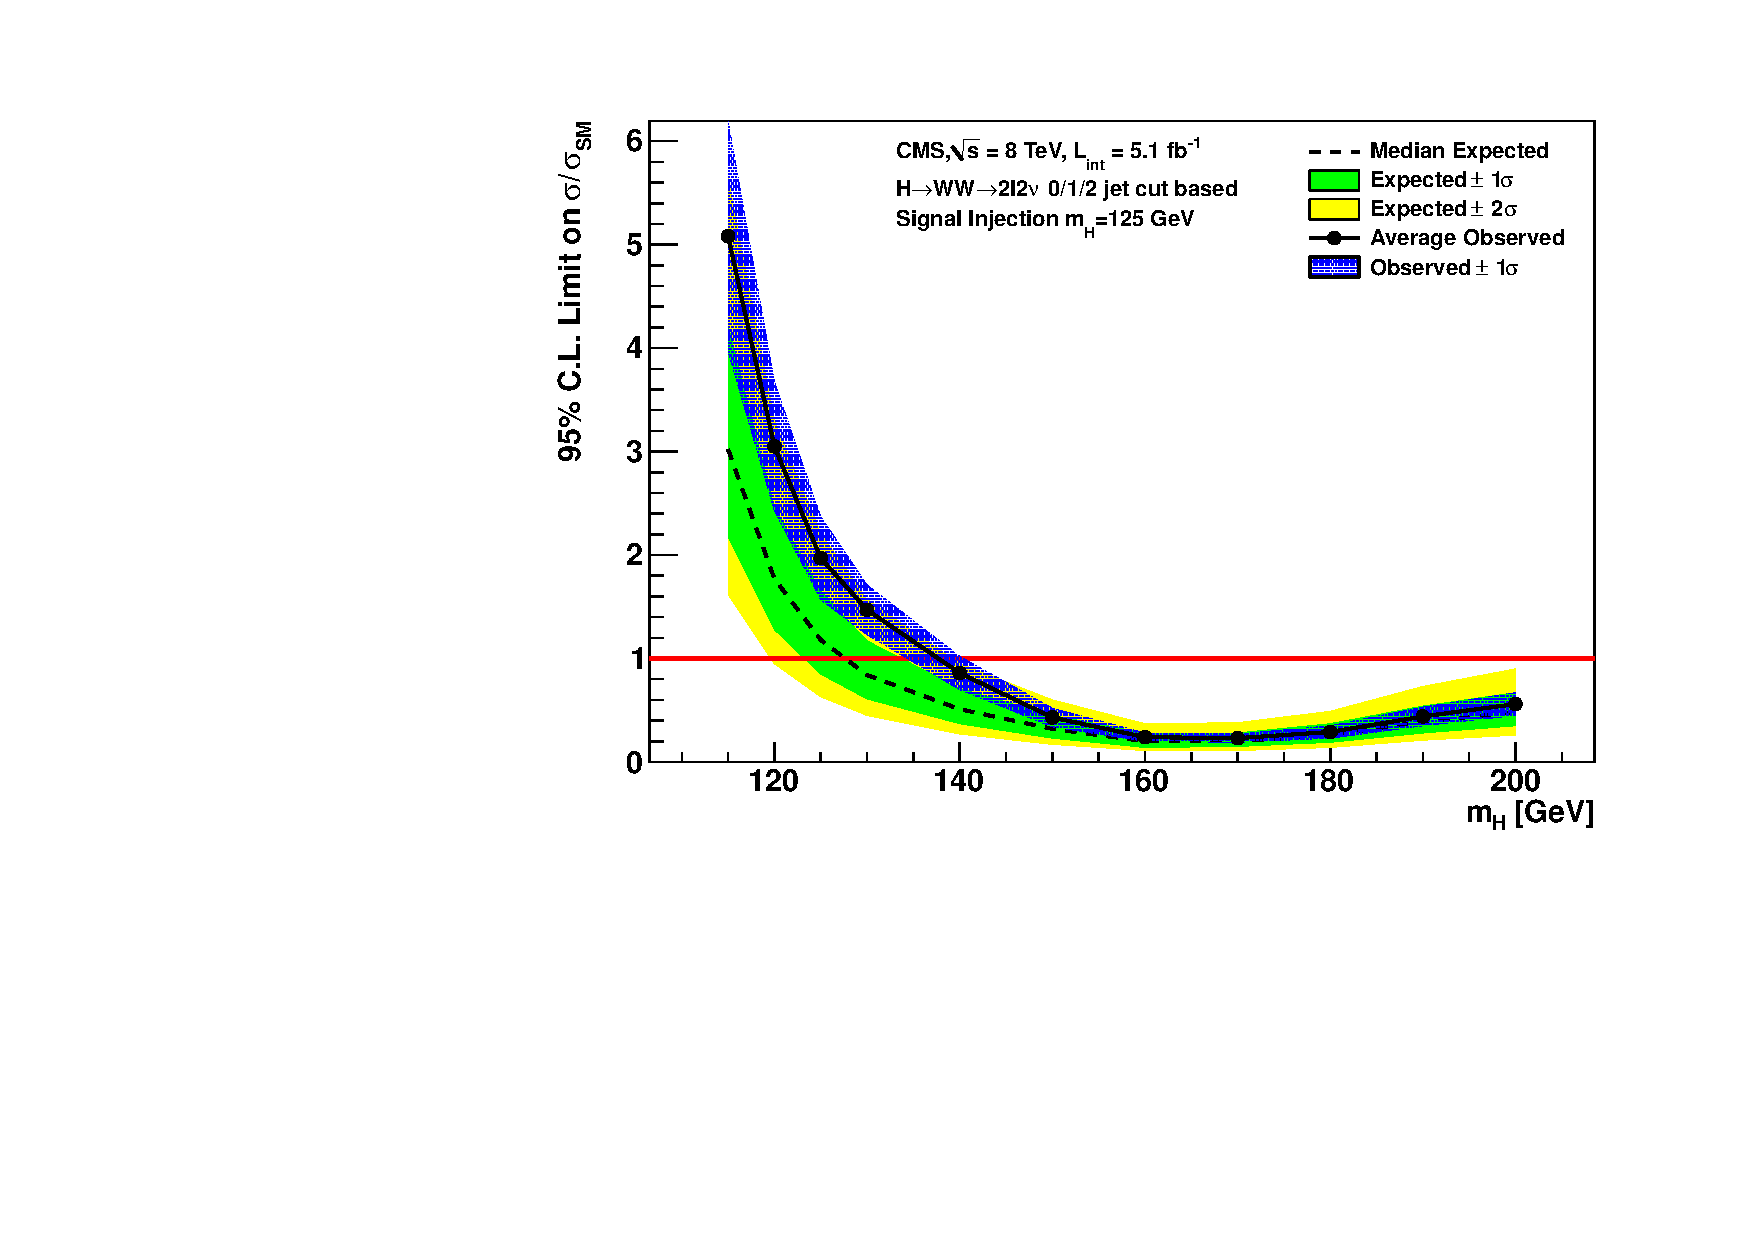
\includegraphics[width=.45\textwidth]{figures/limit_cut_inj125.pdf}
}
\subfigure[cut-based (log Y)]{
\centering
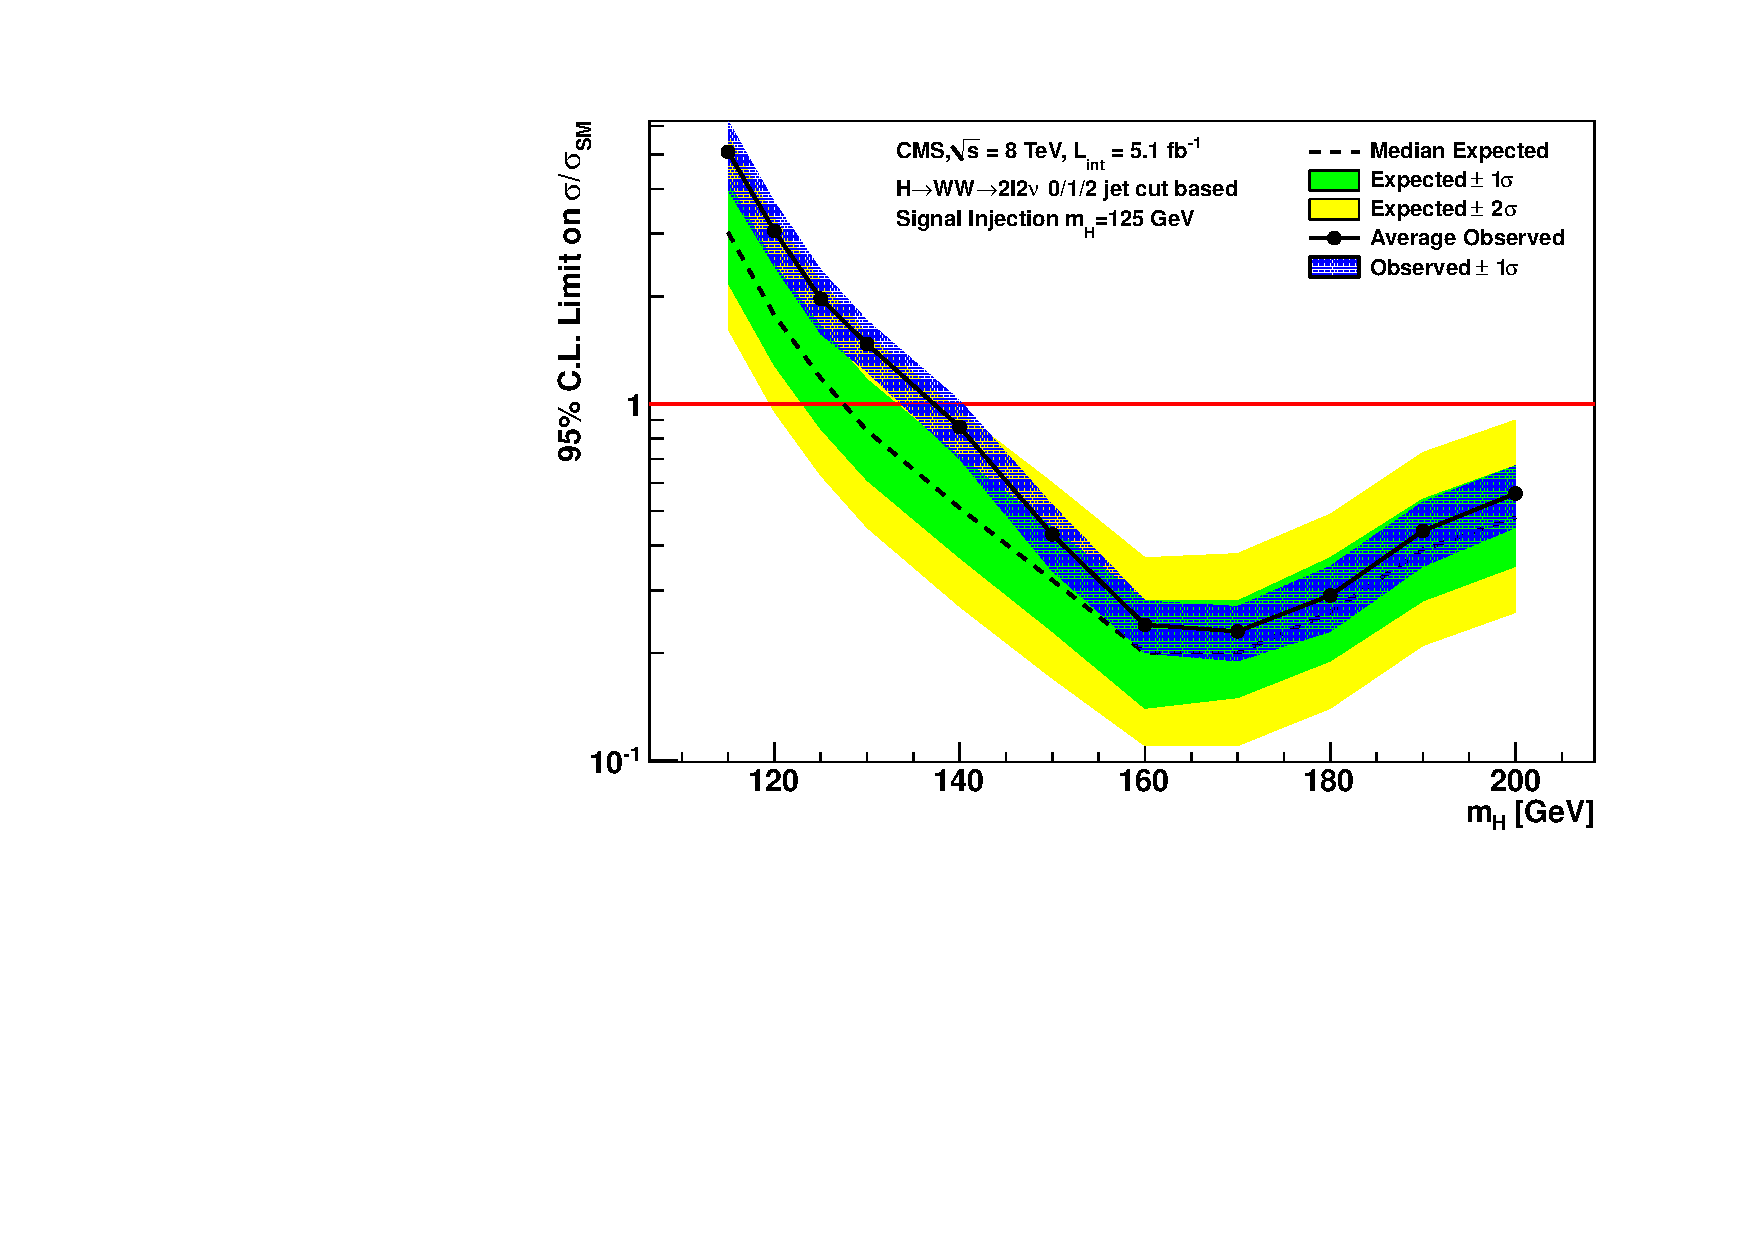
\includegraphics[width=.45\textwidth]{figures/limit_cut_inj125_logy.pdf}
}\\
\centering
\subfigure[shape-based]{
\centering
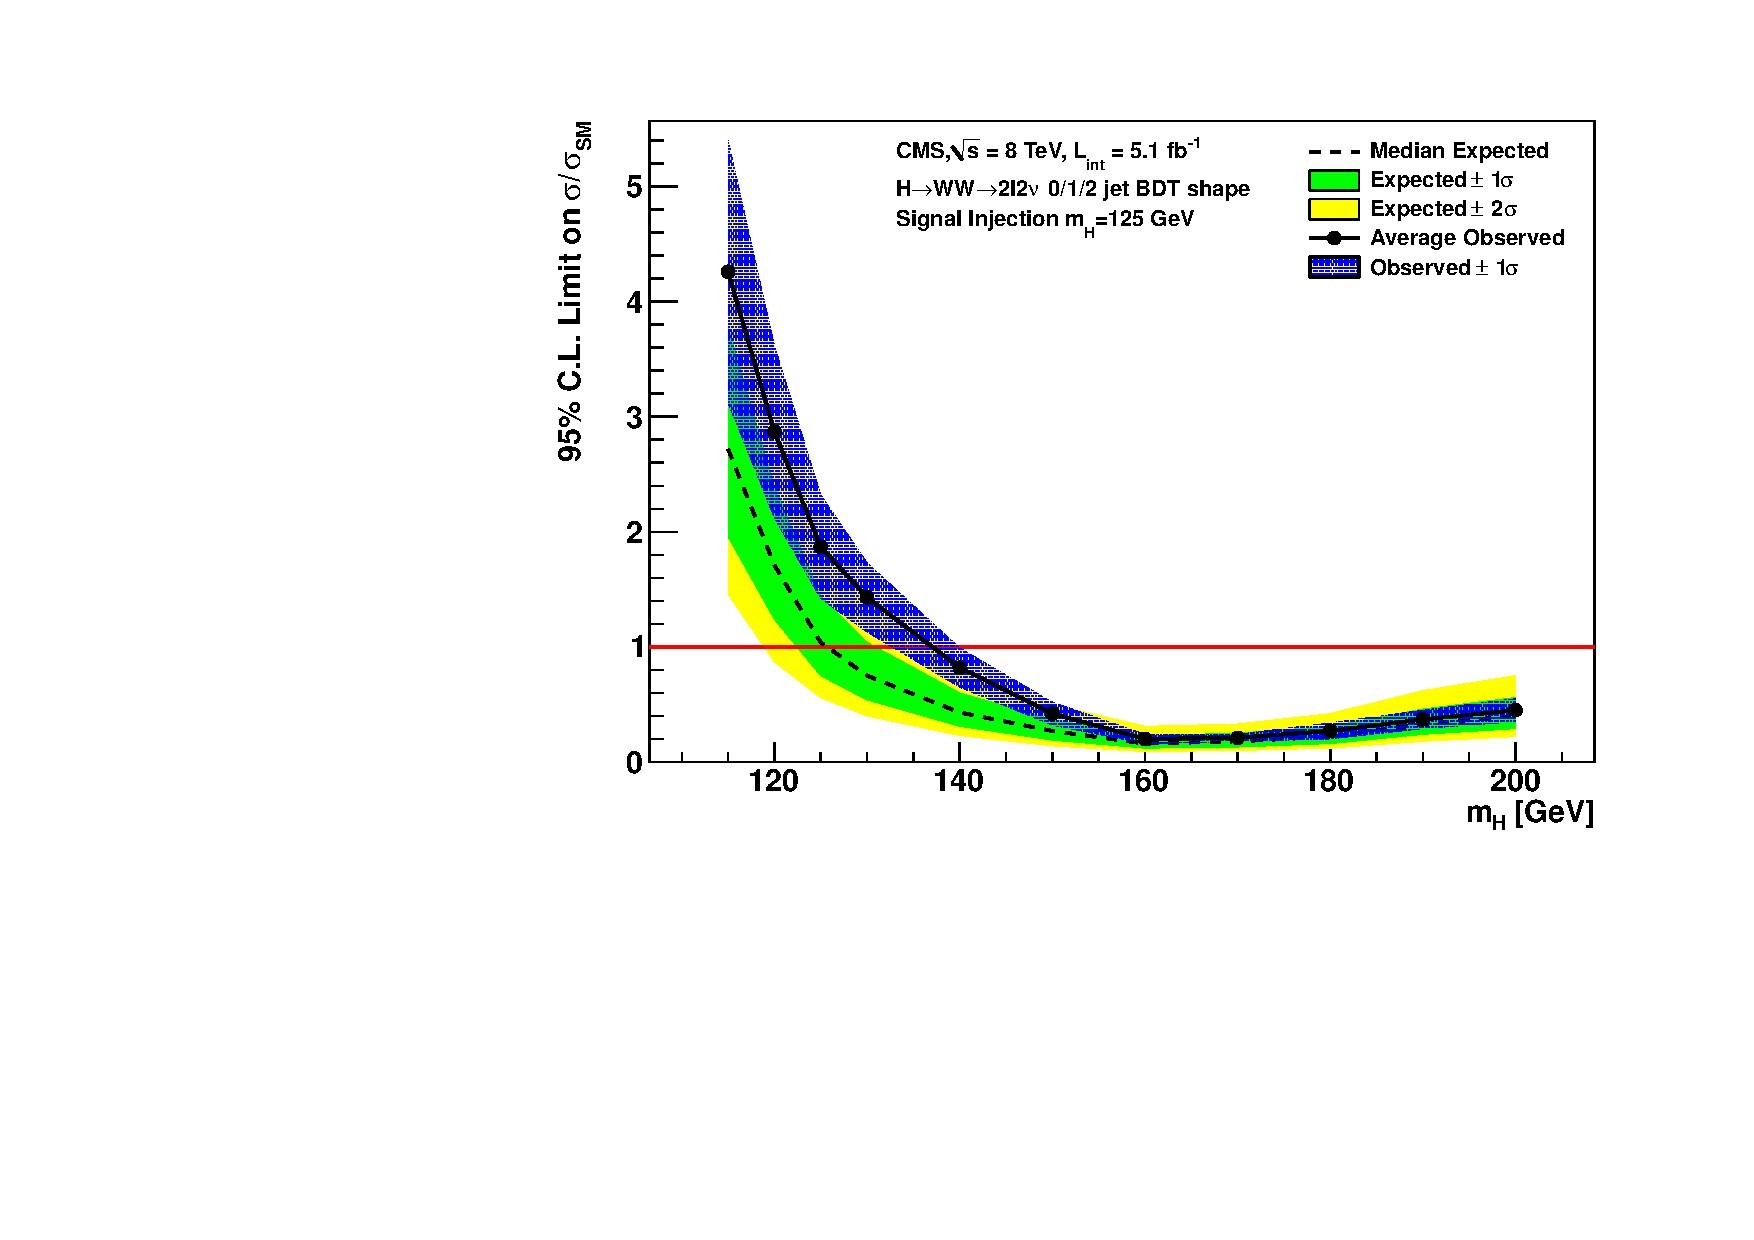
\includegraphics[width=.45\textwidth]{figures/limit_shape_inj125.pdf}
}
\centering
\subfigure[shape-based (log Y)]{
\centering
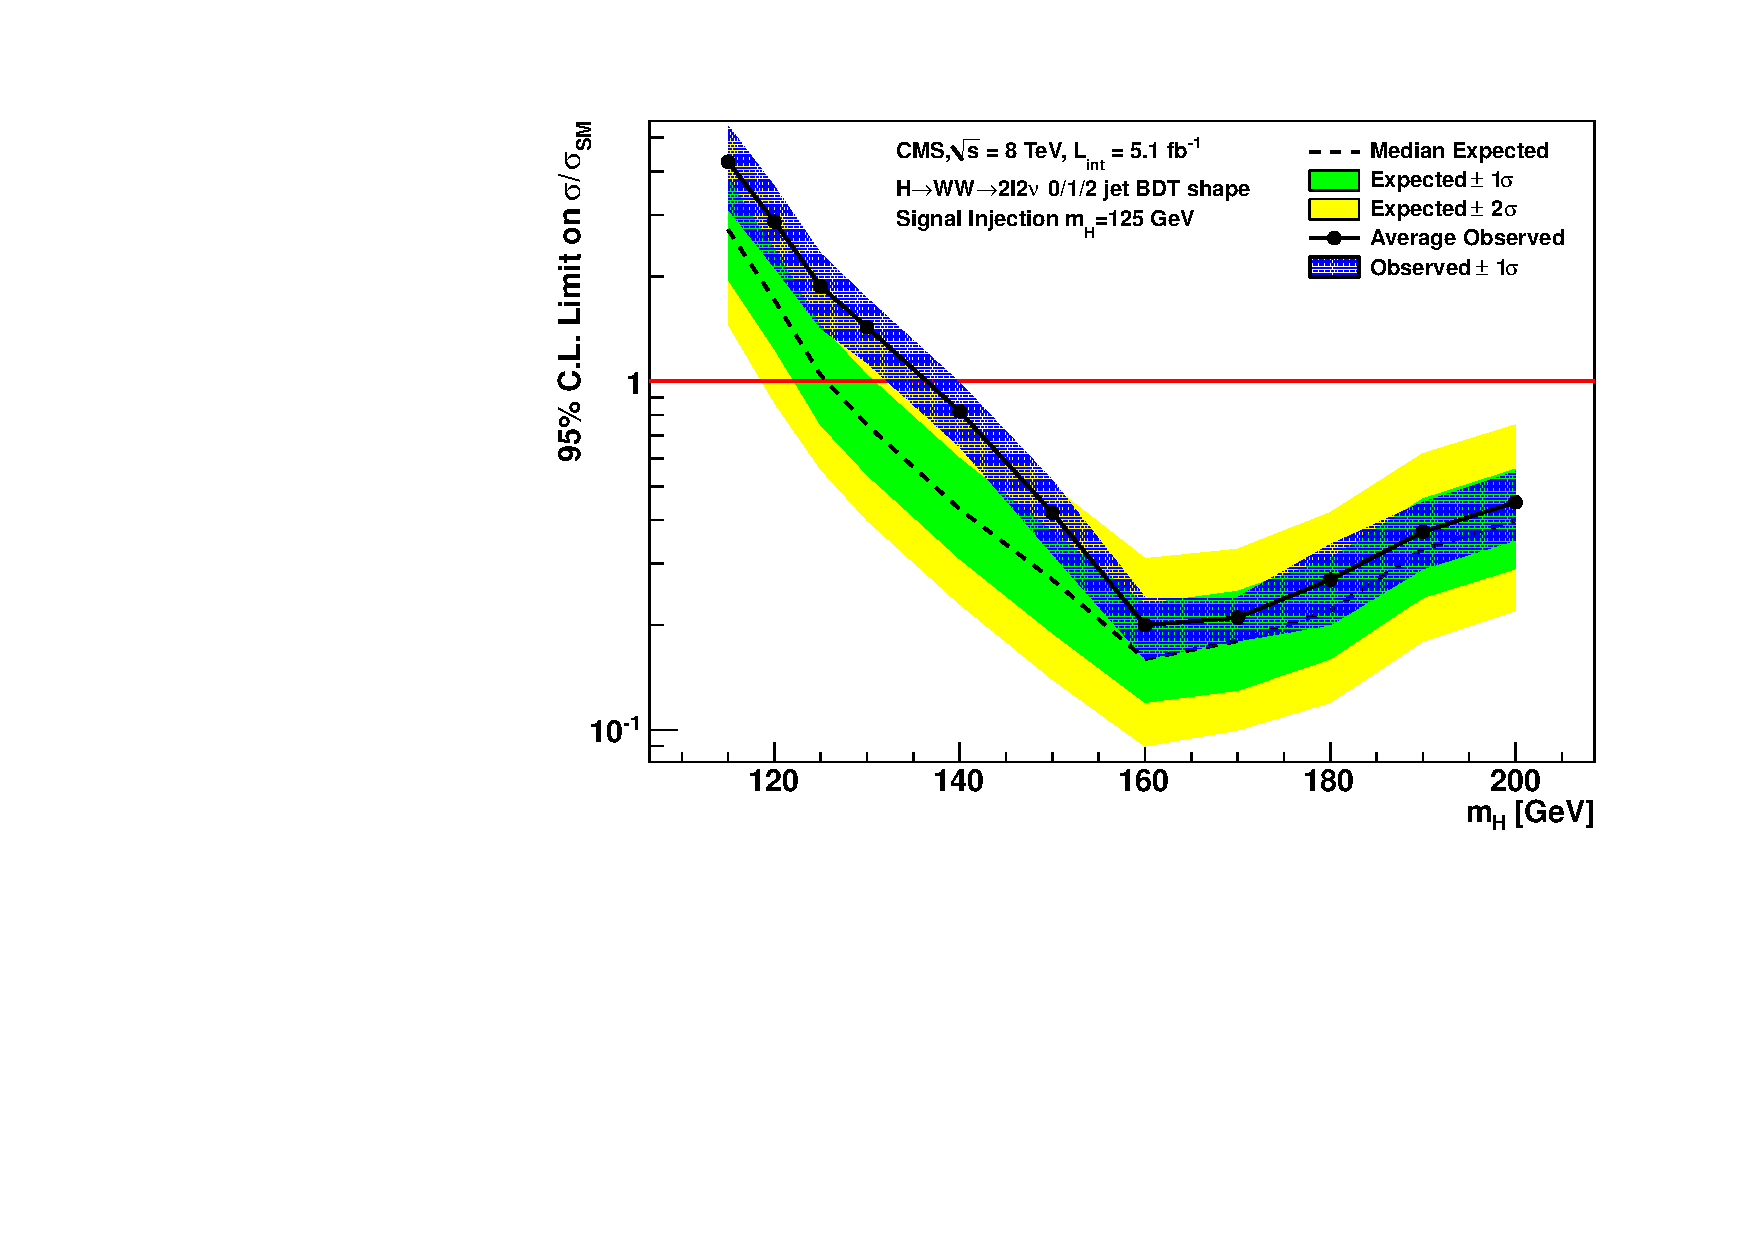
\includegraphics[width=.45\textwidth]{figures/limit_shape_inj125_logy.pdf}
}
\caption{Upper limits in the 0/1/2-jet bins for SM Higgs with 5.1$\ifb$ 
 of data in the case of the presence of a Higgs with $\mHi = 125~\GeV$.
The blue band corresponds to the standard deviation obtained from 
100 toy experiments.}
\label{fig:uls_mh125_nj}
\end{figure}
%%%%%%%%%%%%%%%%%%%%%%%%%%%%%%


%%%%%%%%%%%%%%%%%%%%%%%%%%%%%%
\begin{figure}[!hbtp]
\centering
\subfigure[\mHi=150 \GeVcc\ analysis]{
\centering
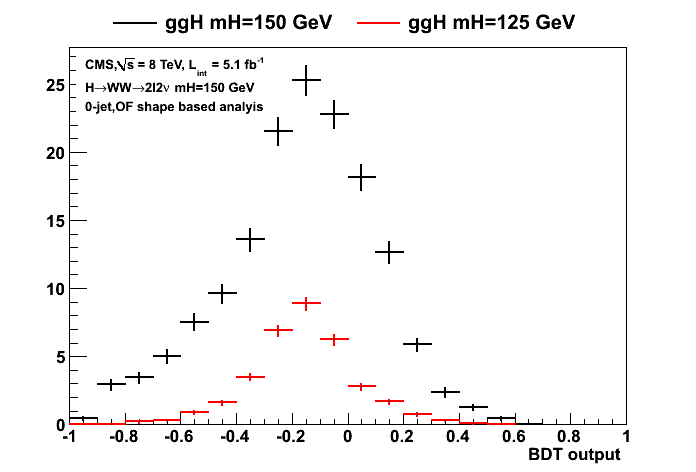
\includegraphics[width=.45\textwidth]{figures/inj125_bdt150.png}
}
\centering
\subfigure[\mHi=160 \GeVcc\ analysis]{
\centering
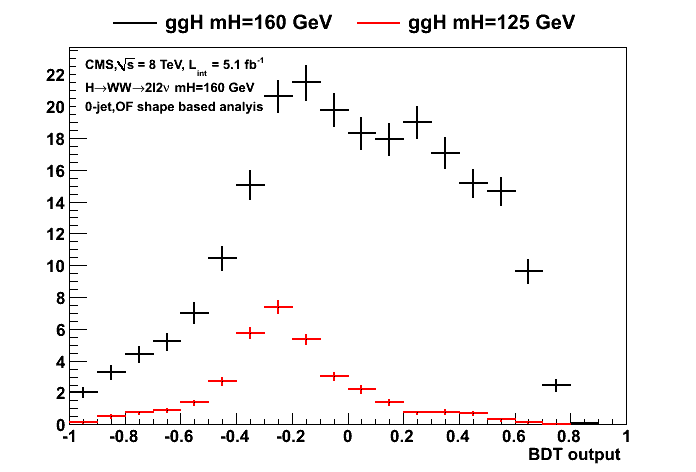
\includegraphics[width=.45\textwidth]{figures/inj125_bdt160.png}
}
\caption{Expected BDT output for a Higgs signal with \mHi=125 and 150 (160) \GeVcc in the 0-jet, OF shape based analysis at  \mHi=150 (160) \GeVcc.}
\label{fig:bdt_mh125}
\end{figure}
%%%%%%%%%%%%%%%%%%%%%%%%%%%%%%

\clearpage

\subsection{8 TeV analysis with 0/1j OF shape based}

%%%%%%%%%%%%%%%%%%%%%%%%%%%%%%
\begin{table}[hbp!]
\begin{center}
\begin{tabular}{c c c c c}
\hline
\vspace{-3mm} && \\
 Higgs Mass & Pseudo-data  & Median expected & Expected range for 68\% & Expected range for 95\%   \\
\vspace{-3mm} && \\
\hline
110 & 5.39$\pm$1.41 & 3.14 & [2.26,  4.36] & [1.68,  5.85] \\
115 & 4.45$\pm$1.19 & 2.81 & [2.03,  3.91] & [1.51,  5.24] \\
120 & 2.86$\pm$0.67 & 1.66 & [1.20,  2.31] & [0.89,  3.10] \\
125 & 1.92$\pm$0.41 & 1.08 & [0.78,  1.50] & [0.58,  2.02] \\
130 & 1.39$\pm$0.28 & 0.78 & [0.56,  1.08] & [0.42,  1.45] \\
140 & 0.81$\pm$0.17 & 0.45 & [0.32,  0.62] & [0.24,  0.84] \\
150 & 0.40$\pm$0.10 & 0.27 & [0.20,  0.38] & [0.15,  0.51] \\
160 & 0.20$\pm$0.04 & 0.17 & [0.12,  0.24] & [0.09,  0.32] \\
170 & 0.20$\pm$0.03 & 0.18 & [0.13,  0.25] & [0.10,  0.34] \\
180 & 0.25$\pm$0.06 & 0.23 & [0.17,  0.32] & [0.12,  0.43] \\
190 & 0.36$\pm$0.09 & 0.34 & [0.24,  0.47] & [0.18,  0.63] \\
200 & 0.45$\pm$0.11 & 0.41 & [0.30,  0.58] & [0.22,  0.77] \\
250 & 0.67$\pm$0.16 & 0.73 & [0.52,  1.01] & [0.39,  1.36] \\
300 & 0.77$\pm$0.21 & 0.85 & [0.61,  1.19] & [0.46,  1.59] \\
\hline
\end{tabular}
\caption{Upper limits in the 0/1/2-jet bins for SM Higgs search using $\intlumiEightTeV$ at 8 TeV 
  in the case of the presence of a Higgs with $\mHi = 125~\GeV$.
  For the 0 and 1 Jet bin final states, the shape based approach is used only in the $e\mu$ channel. 
  The error on the Pseudo-data value corresponds to the standard deviation obtained from 
  100 toy experiments.}
\label{tab:bdtofcutsf_mh125_nj}
\end{center}
\end{table}
%%%%%%%%%%%%%%%%%%%%%%%%%%%%%%

%%%%%%%%%%%%%%%%%%%%%%%%%%%%%%
\begin{figure}[!hbtp]
\centering
\subfigure[linear Y]{
\centering
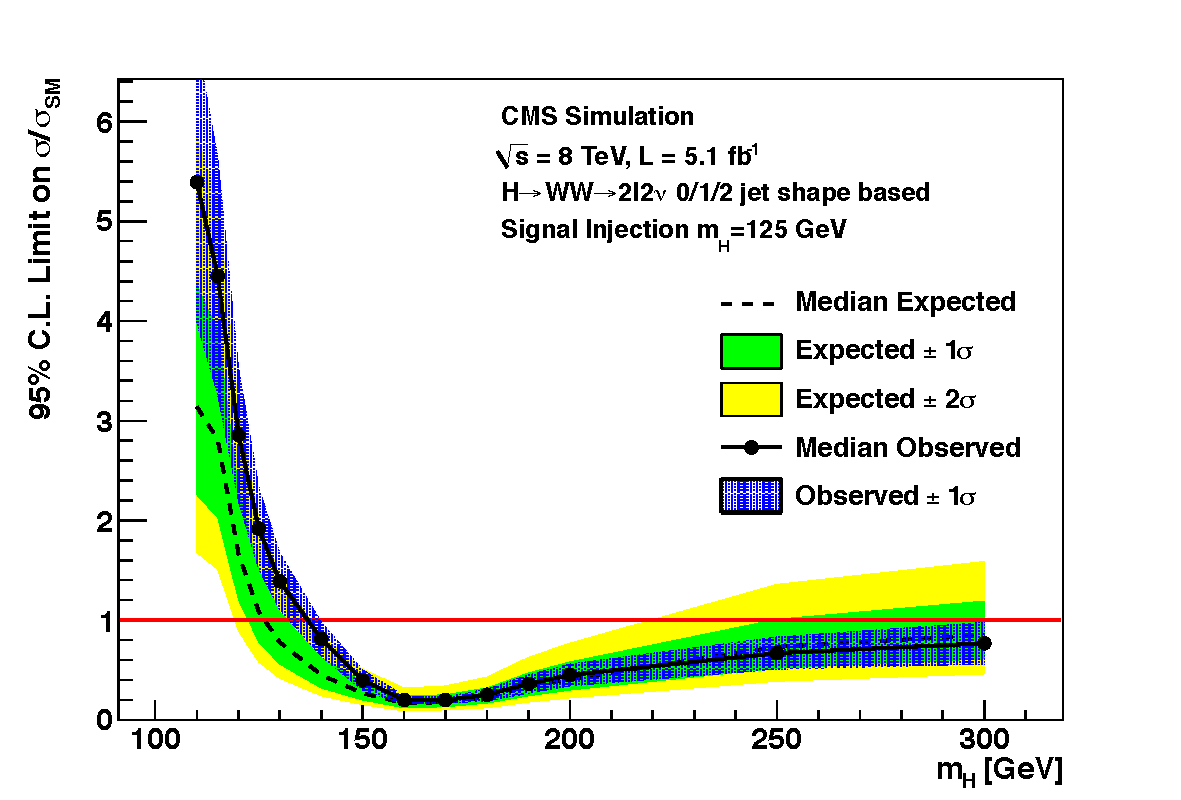
\includegraphics[width=.45\textwidth]{figures/limit_shapeofcutsf_inj125.pdf}
}
\centering
\subfigure[log Y]{
\centering
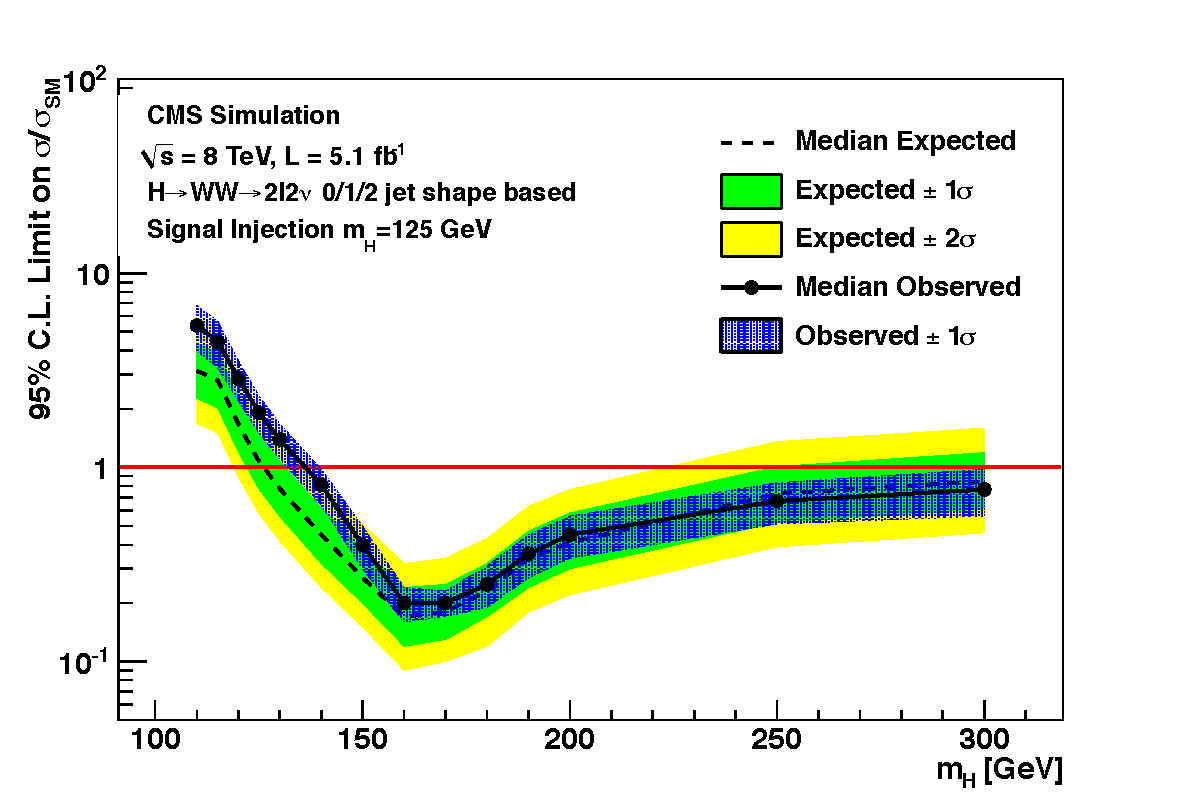
\includegraphics[width=.45\textwidth]{figures/limit_shapeofcutsf_inj125_log.pdf}
}
\caption{Upper limits in the 0/1/2-jet bins for SM Higgs with 5.1$\ifb$ 
 of data in the case of the presence of a Higgs with $\mHi = 125~\GeV$.
 For the 0 and 1 Jet bin final states, the shape based approach is used only in the $e\mu$ channel. 
 The blue band corresponds to the standard deviation obtained from 
 100 toy experiments.}
\label{fig:uls_shapeofcutsf_mh125_nj}
\end{figure}
%%%%%%%%%%%%%%%%%%%%%%%%%%%%%%

\clearpage

\subsection{7 TeV + 8 TeV combination}


%%%%%%%%%%%%%%%%%%%%%%%%%%%%%%
\begin{table}[hbp!]
\begin{center}
\begin{tabular}{c c c c c}
\hline
\vspace{-3mm} && \\
 Higgs Mass & Pseudo-data  & Median expected & Expected range for 68\% & Expected range for 95\%   \\
\vspace{-3mm} && \\
\hline
110 & 8.34$\pm$2.12 & 3.90 & [2.77,  5.43] & [2.06,  7.28] \\
115 & 4.03$\pm$1.17 & 2.07 & [1.49,  2.88] & [1.11,  3.86] \\
120 & 2.62$\pm$0.56 & 1.21 & [0.87,  1.68] & [0.65,  2.25] \\
125 & 1.62$\pm$0.28 & 0.85 & [0.61,  1.18] & [0.45,  1.58] \\
130 & 1.20$\pm$0.24 & 0.58 & [0.42,  0.80] & [0.31,  1.08] \\
140 & 0.67$\pm$0.16 & 0.35 & [0.25,  0.49] & [0.19,  0.65] \\
150 & 0.37$\pm$0.08 & 0.24 & [0.17,  0.33] & [0.13,  0.44] \\
160 & 0.19$\pm$0.03 & 0.16 & [0.11,  0.22] & [0.08,  0.29] \\
170 & 0.19$\pm$0.02 & 0.16 & [0.12,  0.23] & [0.09,  0.30] \\
180 & 0.21$\pm$0.03 & 0.20 & [0.15,  0.28] & [0.11,  0.38] \\
190 & 0.31$\pm$0.09 & 0.29 & [0.21,  0.41] & [0.16,  0.54] \\
200 & 0.41$\pm$0.11 & 0.36 & [0.26,  0.51] & [0.20,  0.68] \\
250 & 0.71$\pm$0.23 & 0.69 & [0.50,  0.96] & [0.37,  1.29] \\
300 & 0.71$\pm$0.21 & 0.75 & [0.54,  1.04] & [0.40,  1.40] \\
\hline
\end{tabular}
\caption{Upper limits in the 0/1/2-jet bins for SM Higgs search
  SM Higgs combining $\intlumiSevenTeV$ at 7 TeV and $\intlumiEightTeV$ at 8 TeV 
  in the case of the presence of a Higgs with $\mHi = 125~\GeV$.
  For the 0 and 1 Jet bin final states, the 7 TeV analysis uses the shape based approach, 
  while the 8 TeV analysis uses the cut based approach. 
  The error on the Pseudo-data value corresponds to the standard deviation obtained from 
  100 toy experiments.}
\label{tab:inj125_nj_comb7shape8cut}
\end{center}
\end{table}
%%%%%%%%%%%%%%%%%%%%%%%%%%%%%%


%%%%%%%%%%%%%%%%%%%%%%%%%%%%%%
\begin{table}[hbp!]
\begin{center}
\begin{tabular}{c c c c c}
\hline
\vspace{-3mm} && \\
 Higgs Mass & Pseudo-data  & Median expected & Expected range for 68\% & Expected range for 95\%   \\
\vspace{-3mm} && \\
\hline
110 & 4.35$\pm$1.53 & 2.67 & [1.92,  3.72] & [1.43,  4.98] \\
115 & 3.66$\pm$1.01 & 1.97 & [1.42,  2.74] & [1.06,  3.68] \\
120 & 2.50$\pm$0.58 & 1.17 & [0.84,  1.62] & [0.63,  2.18] \\
125 & 1.71$\pm$0.35 & 0.80 & [0.57,  1.11] & [0.43,  1.49] \\
130 & 1.23$\pm$0.23 & 0.56 & [0.40,  0.77] & [0.30,  1.04] \\
140 & 0.70$\pm$0.16 & 0.33 & [0.23,  0.45] & [0.17,  0.61] \\
150 & 0.37$\pm$0.09 & 0.22 & [0.16,  0.30] & [0.12,  0.40] \\
160 & 0.17$\pm$0.03 & 0.15 & [0.10,  0.20] & [0.08,  0.27] \\
170 & 0.17$\pm$0.03 & 0.17 & [0.12,  0.24] & [0.09,  0.33] \\
180 & 0.21$\pm$0.05 & 0.19 & [0.14,  0.26] & [0.10,  0.35] \\
190 & 0.30$\pm$0.08 & 0.27 & [0.19,  0.37] & [0.14,  0.50] \\
200 & 0.38$\pm$0.11 & 0.33 & [0.24,  0.46] & [0.18,  0.61] \\
250 & 0.55$\pm$0.19 & 0.58 & [0.42,  0.81] & [0.31,  1.09] \\
300 & 0.57$\pm$0.20 & 0.65 & [0.46,  0.90] & [0.35,  1.20] \\
\hline
\end{tabular}
\caption{Upper limits in the 0/1/2-jet bins for SM Higgs search
  SM Higgs combining $\intlumiSevenTeV$ at 7 TeV and $\intlumiEightTeV$ at 8 TeV 
  in the case of the presence of a Higgs with $\mHi = 125~\GeV$.
  For the 0 and 1 Jet bin final states, the 7 TeV analysis uses the shape based approach for all 
  lepton flavor final states, while the 8 TeV analysis uses the shape based approach only 
  in the $e\mu$ channel. 
  The error on the Pseudo-data value corresponds to the standard deviation obtained from 
  100 toy experiments.}
\label{tab:inj125_nj_comb7shape8shape}
\end{center}
\end{table}
%%%%%%%%%%%%%%%%%%%%%%%%%%%%%%



%%%%%%%%%%%%%%%%%%%%%%%%%%%%%%
\begin{figure}[!hbtp]
\centering
\subfigure[7 TeV shape + 8 TeV cut]{
\centering
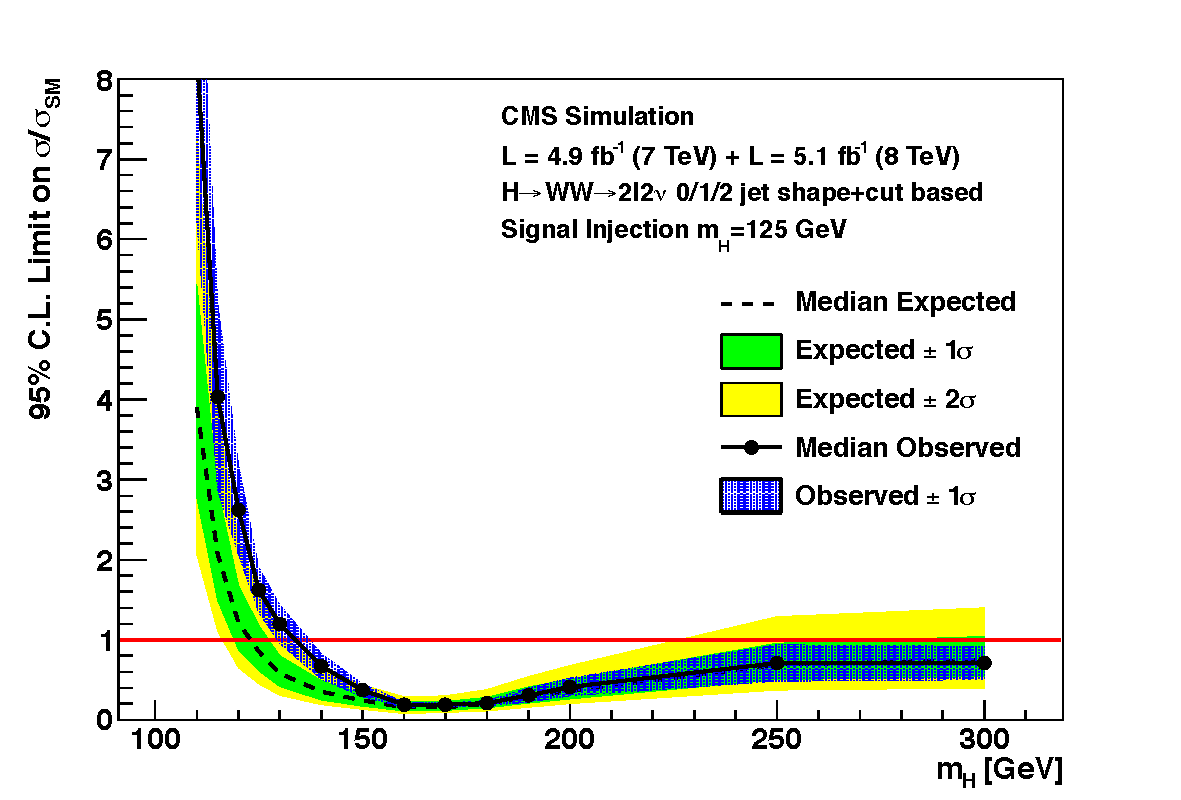
\includegraphics[width=.45\textwidth]{figures/limit_combine7shape8cut_inj125.pdf}
}
\subfigure[7 TeV shape + 8 TeV cut (log Y)]{
\centering
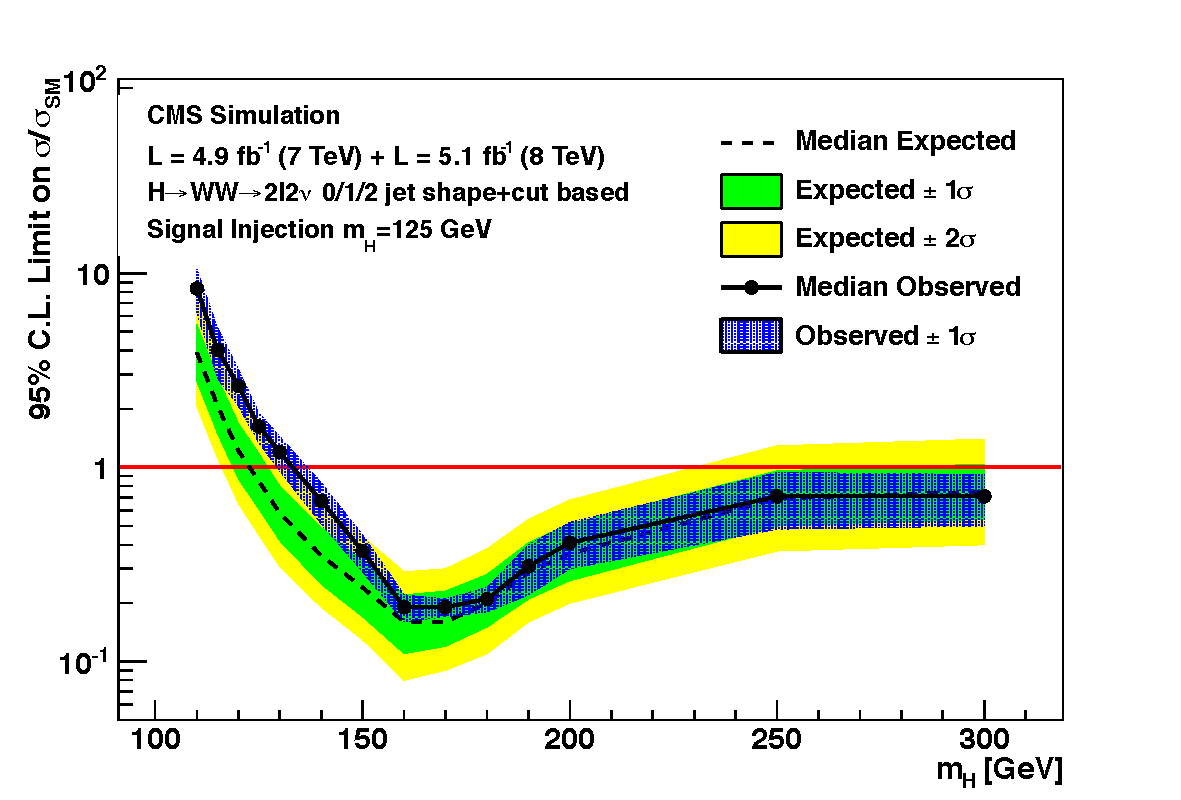
\includegraphics[width=.45\textwidth]{figures/limit_combine7shape8cut_inj125_log.pdf}
}\\
\centering
\subfigure[7 TeV shape + 8 TeV cut/shape]{
\centering
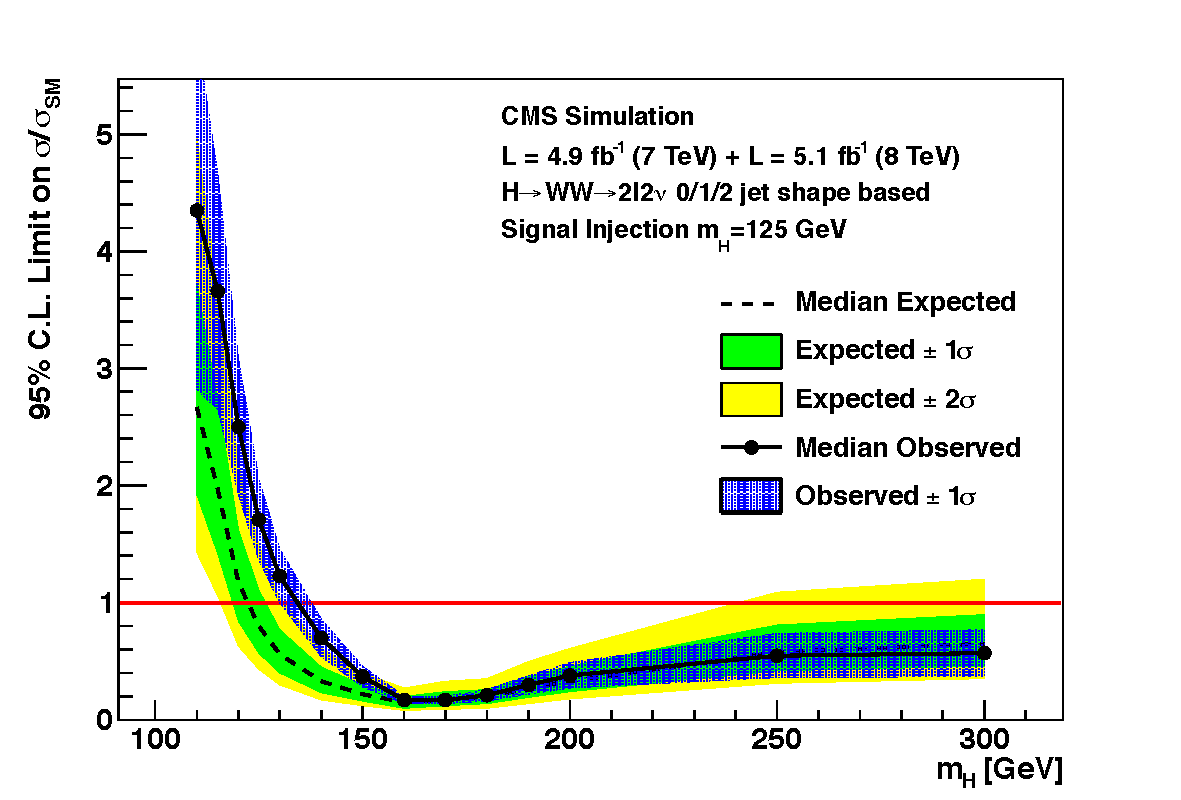
\includegraphics[width=.45\textwidth]{figures/limit_combine7shape8shape_inj125.pdf}
}
\centering
\subfigure[7 TeV shape + 8 TeV cut/shape (log Y)]{
\centering
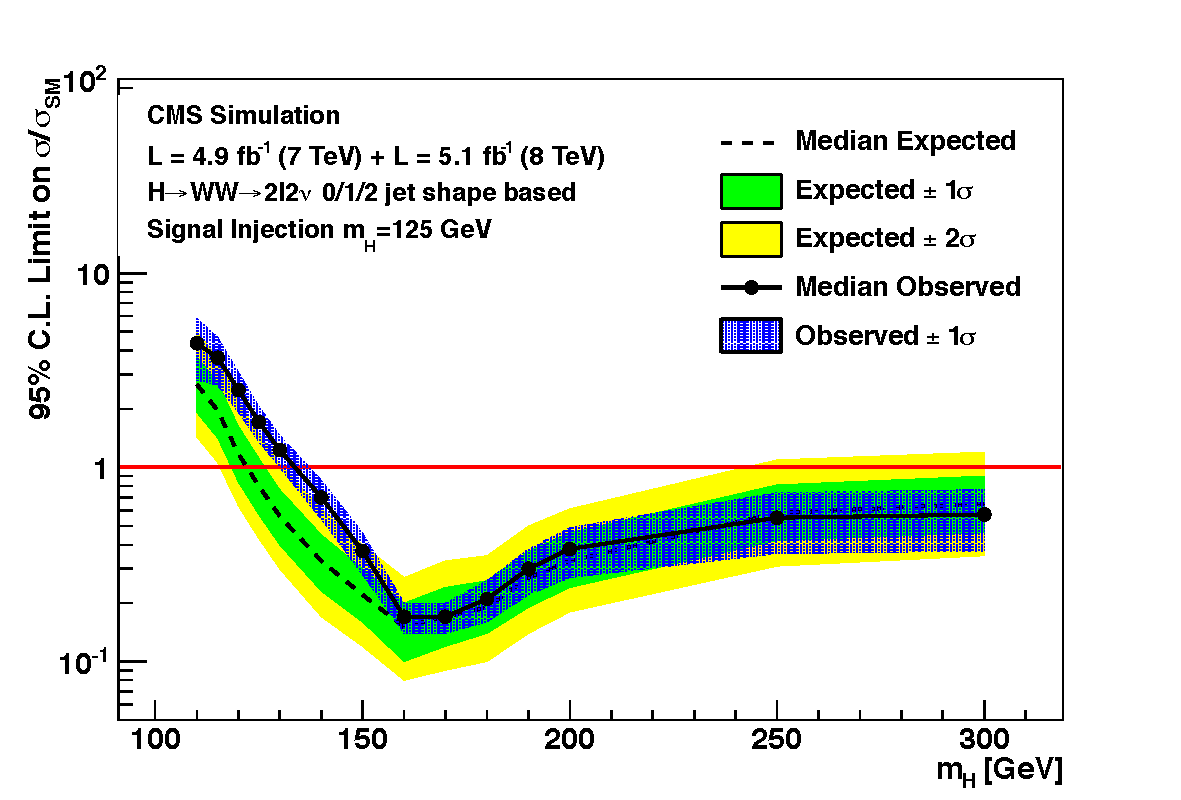
\includegraphics[width=.45\textwidth]{figures/limit_combine7shape8shape_inj125_log.pdf}
}
\caption{Upper limits in the 0/1/2-jet bins for SM Higgs search
  SM Higgs combining $\intlumiSevenTeV$ at 7 TeV and $\intlumiEightTeV$ at 8 TeV 
  in the case of the presence of a Higgs with $\mHi = 125~\GeV$.
  For the 0 and 1 Jet bin final states, the 7 TeV analysis uses the shape based approach for all 
  lepton flavor final states, while the 8 TeV analysis uses the shape based approach only 
  in the $e\mu$ channel. 
  The blue band corresponds to the standard deviation obtained from 
  100 toy experiments.}
\label{fig:uls_mh125_nj_comb}
\end{figure}
%%%%%%%%%%%%%%%%%%%%%%%%%%%%%%

